\chapter{Background teorico}
\label{cap:background}

Per inquadrare le scelte progettuali descritte nei capitoli successivi è utile richiamare brevemente i concetti teorici alla base del sistema: la struttura di una pipeline ALPR, le reti neurali convoluzionali utilizzate per la localizzazione di oggetti, l'architettura dei Vision Transformer nella variante compatta, e le tecniche di quantizzazione che rendono possibile l'esecuzione di tali reti su microcontrollori.

\section{Pipeline ALPR a due stadi}
\label{sec:alpr-pipeline}

Il riconoscimento automatico delle targhe viene generalmente organizzato in due stadi. Il primo, detto \textit{detection}, localizza nell'immagine la regione contenente la targa e restituisce il relativo \textit{bounding box}. Il secondo, detto \textit{Optical Character Recognition} (OCR), riceve il ritaglio prodotto dal detector e ne estrae la sequenza alfanumerica. Questa separazione consente di affrontare con modelli diversi due problemi distinti, individuare la targa e leggerne il contenuto e, nel contesto embedded del progetto, permette di distribuire il carico di lavoro su due schede separate.

 
\begin{figure}[H]
    \centering
    \begin{tikzpicture}[
        font=\footnotesize,
        stage/.style={
            draw, thick, rounded corners=3pt,
            inner sep=4pt,
            fill=custom_lightgray,
            align=center
        },
        arrow/.style={
            ->, >=stealth, very thick, custom_blue
        },
        label/.style={
            font=\scriptsize\bfseries,
            align=center
        }
    ]
 
        % -------- BOX 1: Input --------
        \node[stage] (input) {
            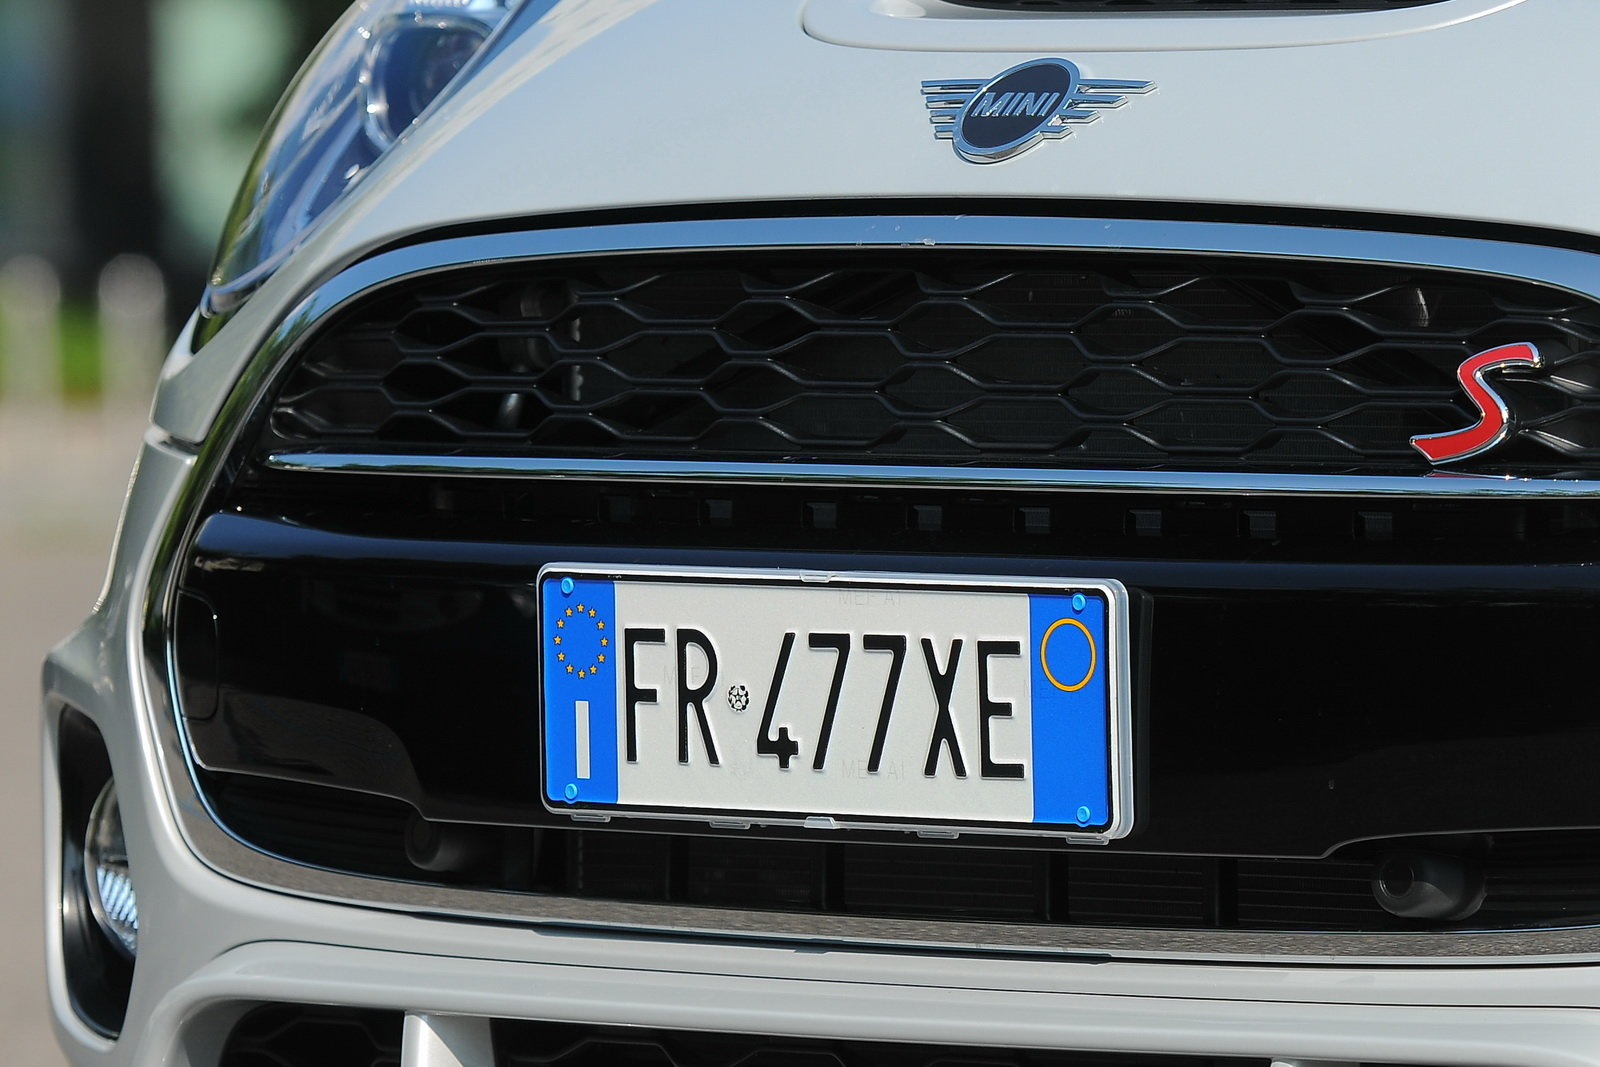
\includegraphics[width=3.5cm]{images/plate_23.jpg}\\[2pt]
            \scriptsize Immagine in ingresso\\
            \scriptsize $192 \times 192$ grayscale
        };
 
        % -------- BOX 2: Detection --------
        \node[stage, right=1.2cm of input] (det) {
            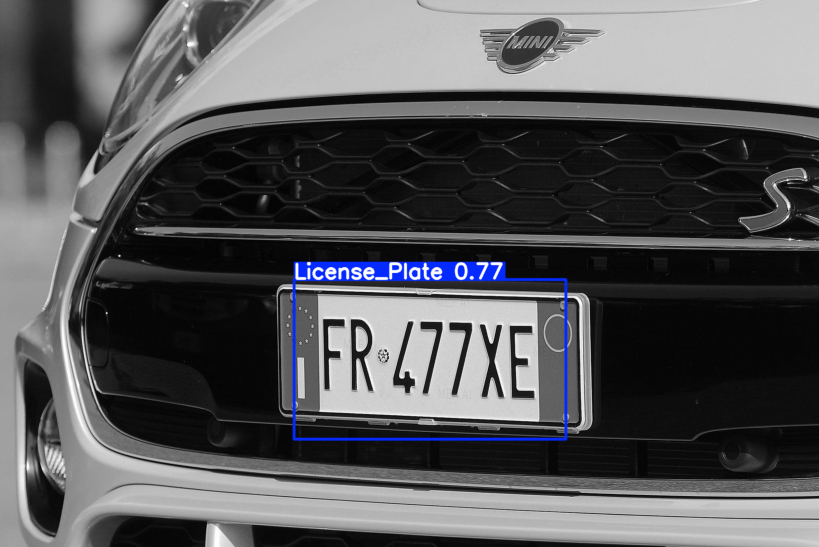
\includegraphics[width=3.5cm]{images/taega_boundingbox.png}\\[2pt]
            \scriptsize Detection (YOLO)\\
            \scriptsize bounding box della targa
        };
 
        % -------- BOX 3: OCR --------
        \node[stage, right=1.2cm of det] (ocr) {
            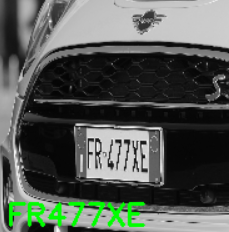
\includegraphics[width=3.0cm]{images/targa_esempio.png}\\[2pt]
            \scriptsize OCR (CCT-XS)\\
            \scriptsize testo decodificato
        };
 
        % -------- Frecce tra i box --------
        \draw[arrow] (input) -- node[above, label, custom_blue] {\tiny Stadio 1} (det);
        \draw[arrow] (det)   -- node[above, label, custom_blue] {\tiny Stadio 2} (ocr);
 
    \end{tikzpicture}
    \caption{Rappresentazione visiva della pipeline ALPR a due stadi.}
    \label{fig:pipeline-visiva}
\end{figure}


\section{Reti neurali per object detection: YOLO}
\label{sec:yolo}

Le reti neurali convoluzionali (\textit{Convolutional Neural Networks}, CNN) sono lo strumento standard per problemi di visione artificiale e si basano su uno schema gerarchico in cui ogni livello apprende rappresentazioni progressivamente più astratte a partire dai pixel grezzi. La famiglia di modelli YOLO (\textit{You Only Look Once})~\cite{redmon_2016_yolo} ha introdotto un approccio unificato al problema della detection: anziché applicare un classificatore su un insieme di proposte di regione, YOLO formula la detection come un unico problema di regressione, in cui una singola rete predice contemporaneamente posizioni e classi di tutti gli oggetti presenti nell'immagine.

La versione utilizzata in questo progetto è \textbf{YOLOv8}~\cite{jocher_2023_yolov8}, sviluppata e mantenuta da Ultralytics. Rispetto alle versioni precedenti, YOLOv8 introduce un \textit{backbone} basato su moduli C2f (Cross-Stage Partial con due flussi paralleli), un \textit{neck} di tipo PAN (\textit{Path Aggregation Network}) per la fusione di feature multi-scala, e una \textit{head} di tipo \textit{anchor-free} che predice direttamente le coordinate dei bounding box senza ricorrere a prior fissati. L'architettura è organizzata in tre uscite di rilevamento corrispondenti a tre scale spaziali differenti, consentendo di catturare oggetti di dimensioni eterogenee. Per ogni anchor della griglia di output, la rete predice quattro valori che descrivono il bounding box (centro e dimensioni) e un valore di confidenza per ciascuna classe. Nel caso di una rete a singola classe, come quella di questo progetto, l'output è dunque costituito da un tensore di forma $[1, 4, N]$ per i bounding box e $[1, 1, N]$ per le confidenze, dove $N$ è il numero totale di anchor che dipende dalle dimensioni dell'immagine in input.

\subsection{Non-Maximum Suppression}
\label{sec:nms}

Dopo l'inferenza, la rete restituisce tipicamente molte detection sovrapposte che si riferiscono allo stesso oggetto. La \textit{Non-Maximum Suppression} (NMS) è la procedura standard per ridurre tali duplicati a una singola predizione per oggetto. L'algoritmo seleziona la detection con confidenza massima e scarta tutte le altre che presentano un'\textit{Intersection over Union} (IoU) superiore a una soglia prefissata. L'IoU tra due bounding box $A$ e $B$ è definita come:
\[
\text{IoU}(A, B) = \frac{|A \cap B|}{|A \cup B|}
\]
e rappresenta il rapporto tra l'area di intersezione e quella di unione. Tipicamente si scartano box con IoU oltre $0{,}5$, ritenendo che facciano riferimento al medesimo oggetto.
\vspace{1.0cm}

\begin{figure}[H]
    \centering
    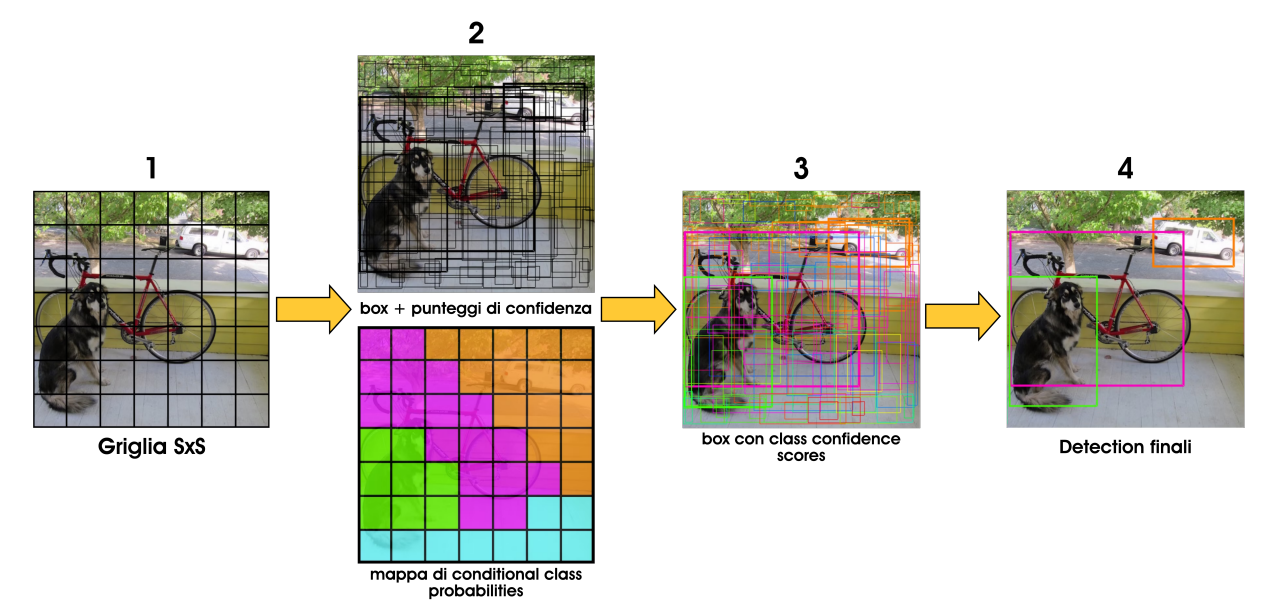
\includegraphics[width=1.0\textwidth]{images/inferenza_yolov8.png}
    \caption{Step della fase di inferenza nelle reti YOLO}
    \label{fig:inferenza yolov8}
\end{figure}


\newpage
\section{Vision Transformer e Compact Convolutional Transformer}
\label{sec:vit-cct}

\iffalse
I \textbf{Vision Transformer} (ViT) sono una classe di modelli che applica l'architettura Transformer, originariamente sviluppata per il \textit{Natural Language Processing}, al dominio delle immagini. L'idea di base è suddividere l'immagine in \textit{patch} non sovrapposte, proiettarle in uno spazio di embedding e processarle come una sequenza di token attraverso un meccanismo di \textit{self-attention} che permette a ciascun token di interagire con tutti gli altri.

Il vantaggio dei ViT rispetto alle CNN consiste nella capacità di modellare relazioni a lungo raggio direttamente, senza dipendere dalla gerarchia di livelli convoluzionali. Lo svantaggio principale è la necessità di grandi quantità di dati di addestramento, poiché il modello dispone di pochissimi bias induttivi (a differenza delle CNN, che hanno la \textit{translation invariance} integrata nella struttura). Inoltre, le architetture ViT originali richiedono milioni di parametri e sono difficilmente eseguibili su hardware con risorse limitate.

Per risolvere questi problemi, Hassani et al.~\cite{hassani_2021_cct} hanno proposto il \textbf{Compact Convolutional Transformer} (CCT), un'architettura ibrida che combina i vantaggi delle CNN e dei Transformer. Le differenze principali rispetto al ViT sono due. Anzitutto, l'embedding iniziale delle patch viene sostituito da un piccolo \textit{convolutional tokenizer}: alcuni strati convoluzionali estraggono feature locali dall'immagine e producono i token di ingresso del Transformer, restituendo a buon mercato i bias induttivi tipici delle CNN. In secondo luogo, il classificatore finale impiega un meccanismo di \textit{sequence pooling} che aggrega l'intera sequenza di token tramite attenzione, anziché utilizzare il token \texttt{[CLS]} dedicato come nel ViT originale.

Il risultato è un modello che mantiene la capacità rappresentazionale dei Transformer ma con un numero di parametri significativamente ridotto e una migliore efficienza di addestramento su dataset di dimensioni contenute. La variante \textbf{CCT-XS} utilizzata in questo progetto è la versione di scala più piccola della famiglia, particolarmente adatta a contesti embedded.
\fi

I \textbf{Vision Transformer} (ViT) applicano l'architettura Transformer, nata per il task di NLP, al dominio delle immagini, suddividendo l'immagine in patch e processandole come sequenze di token tramite \textit{self-attention}. Rispetto alle CNN, i ViT modellano relazioni a lungo raggio più efficacemente, ma richiedono grandi quantità di dati e molti parametri, risultando difficilmente adattabili a hardware con risorse limitate. Per ovviare a questi limiti, Hassani et al.~\cite{hassani_2021_cct} hanno proposto il \textbf{Compact Convolutional Transformer} (CCT), un'architettura ibrida che sostituisce l'embedding iniziale delle patch con un \textit{convolutional tokenizer} grazie al quale alcuni strati convoluzionali estraggono feature locali dall'immagine e producono i token di ingresso del Transformer. In secondo luogo, il classificatore finale impiega un meccanismo di \textit{sequence pooling} che aggrega l'intera sequenza di token tramite attenzione, anziché utilizzare il token \texttt{[CLS]} dedicato come nel ViT originale. Il risultato è un modello compatto, con un numero di parametri significativamente ridotto rispetto al ViT originale e una migliore efficienza di addestramento su dataset di dimensioni contenute.

Nel presente progetto, il CCT non è stato addestrato direttamente. La variante \texttt{CCT-XS}, la versione di scala più piccola della famiglia, è l'architettura alla base di una repository open-source individuata per il modulo OCR su targhe automobilistiche \cite{ankandrew_2024_fastplateocr}. Da essa sono stati ereditati sia i pesi pre-addestrati sul riconoscimento di caratteri sia la struttura di inferenza, che è stata successivamente adattata e quantizzata per il deployment sulla Board B. La scelta di questa architettura si è rivelata adeguata al contesto embedded grazie alle sue dimensioni contenute e alla buona accuratezza sul riconoscimento di sequenze alfanumeriche tipiche delle targhe automobilistiche.
\begin{figure}[H]
    \centering
    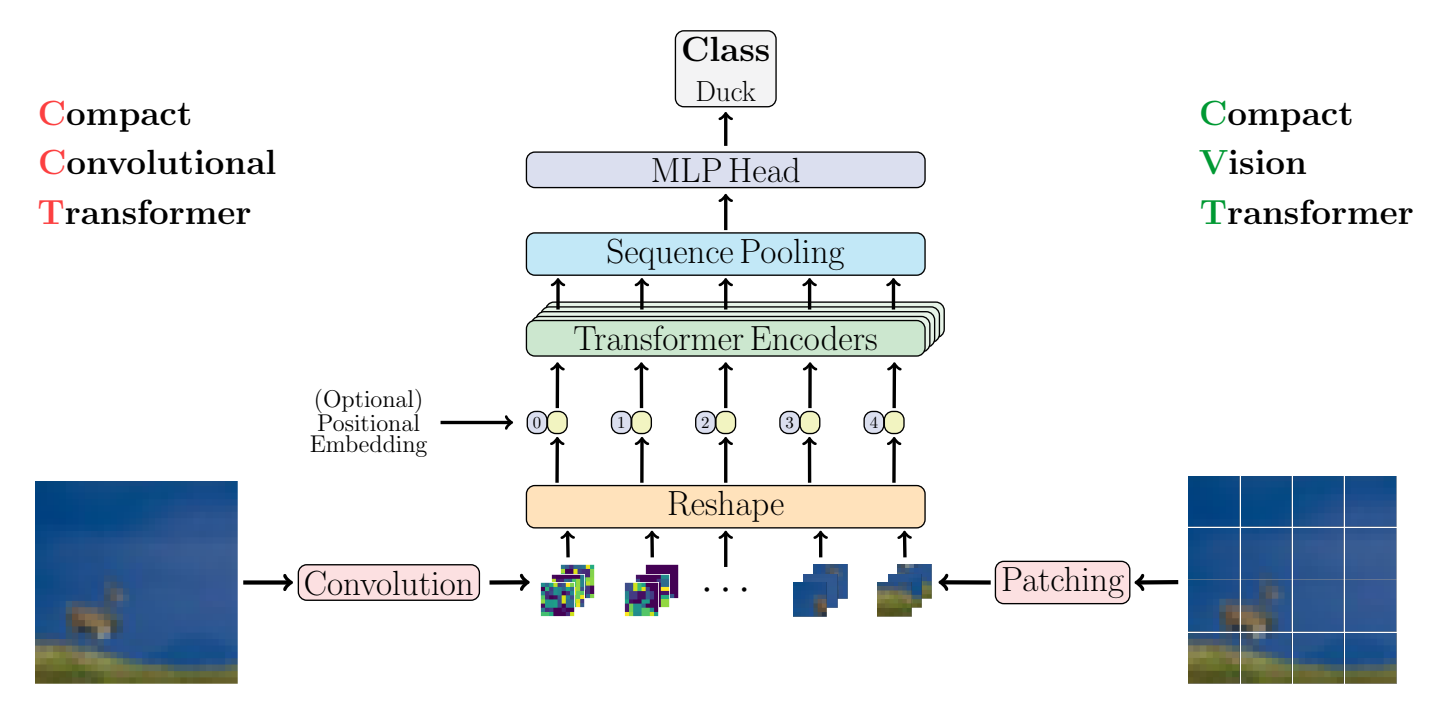
\includegraphics[width=0.9\textwidth]{images/cvtransofrmer.png}
    \caption{Architettura proposta nel paper "\textit{Escaping the Big Data Paradigm with
Compact Transformers}"}
    \label{fig:architettura-cct}
\end{figure}

\section{Quantizzazione INT8 e X-CUBE-AI}
\label{sec:quantization}

I modelli neurali sono tipicamente addestrati in aritmetica a virgola mobile a 32 bit (FP32). Tuttavia, per l'esecuzione su microcontrollori questo formato è inefficiente sia in termini di memoria (i pesi occupano 4 byte ciascuno) sia di prestazioni, perché molti microcontrollori non possiedono unità SIMD per il calcolo vettoriale in floating point. La tecnica della \textbf{quantizzazione} consiste nel rappresentare i pesi e le attivazioni della rete con interi a precisione ridotta, tipicamente 8 bit~\cite{jacob_2018_quantization}, riducendo l'occupazione di memoria di un fattore quattro e abilitando l'uso di istruzioni intere veloci.

\begin{boxH}
La quantizzazione INT8 con \textit{scale} e \textit{zero-point} è la forma più comune e mappa un valore reale $r$ su un intero $q$ a 8 bit tramite la relazione:
\textbf{\[
r = (q - z) \cdot s
\]}
\end{boxH}
dove $s$ (scale) è un fattore di scala in virgola mobile e $z$ (zero-point) è un offset intero. I parametri $s$ e $z$ vengono determinati separatamente per ciascun tensore della rete a partire da un piccolo insieme di campioni di calibrazione che permette di stimare l'intervallo dinamico dei valori. La conversione finale dell'output da intero a reale, detta \textit{dequantizzazione}, è dunque un'operazione esplicita che viene effettuata in software dopo l'inferenza, prima dell'applicazione di soglie o funzioni non lineari come la softmax.

In questo progetto la quantizzazione è affidata a \textbf{X-CUBE-AI} di STMicroelectronics~\cite{stm32cubeai_doc}, che importa il modello ONNX, applica la quantizzazione post-training e genera una libreria C ottimizzata per STM32. Il codice prodotto espone inoltre i parametri \texttt{SCALE} e \texttt{ZERO\_POINT}, necessari per quantizzare gli input e dequantizzare gli output dell'inferenza.

\section{Zephyr come sistema operativo embedded}
\label{sec:zephyr}

\textbf{Zephyr}~\cite{zephyr_doc} è un sistema operativo real-time open source pensato per dispositivi con risorse limitate. Nel progetto è stato scelto per la sua modularità, basata su KConfig e devicetree, che consente di includere solo i componenti necessari e di descrivere l'hardware in modo separato dal codice applicativo. Rispetto ad alternative come HAL o FreeRTOS, Zephyr offre driver già pronti e una configurazione più flessibile della piattaforma STM32H7. In particolare, sono risultati decisivi il supporto alla UART interrupt-driven, la possibilità di riconfigurare la SRAM tramite overlay devicetree e la compatibilità con la FPU hard-float richiesta dalla libreria X-CUBE-AI.

\begin{figure}[H]
    \centering
    
\includegraphics[width=0.3\textwidth]{images/logo_zephyt.png}
    \caption{Logo di \textit{Zephyr OS}.}
    \label{fig:zephyr os}
\end{figure}
